% figure: 自控-典型二阶系统结构图.png
% 用途：自控 05-3-b-2 例5-13 —— 典型二阶系统（教材图5-41）
% 构建：..\build.ps1 -File .\block-2nd-order.tex
\documentclass[border=10pt]{standalone}
\usepackage{fontspec}
\setmainfont{Cambria}
\usepackage{unicode-math}
\setmathfont{Cambria Math}
\usepackage{tikz}
\usetikzlibrary{positioning, arrows.meta, calc}
\usepackage{ctex}

\definecolor{figink}{HTML}{1E2228}
\definecolor{figacc}{HTML}{B23020}
\definecolor{figfill}{HTML}{E8EFF8}
\definecolor{figsub}{HTML}{606874}

\begin{document}
\begin{tikzpicture}[
  x=1cm, y=1cm,
  line width=0.95pt, line cap=round, line join=round,
  >=Stealth,
  blk/.style = {draw=figink, line width=0.95pt, fill=figfill,
                minimum width=3.6cm, minimum height=1.05cm, inner sep=3pt,
                anchor=center, font=\small, align=center},
  sum/.style = {draw=figink, line width=0.95pt, circle, inner sep=0pt,
                minimum size=0.42cm, anchor=center},
  sig/.style = {font=\small, color=figink, fill=white},
  lbl/.style = {font=\small, inner sep=1.5pt, fill=white},
  sub/.style = {font=\footnotesize, color=figsub, fill=white}
]

\node[sum] (s1) at (0,0) {};
\node[blk] (g)  at (3.4,0) {$\dfrac{\omega_n^{2}}{s\,(s+2\zeta\omega_n)}$\\[3pt]
                            {\footnotesize 典型二阶对象}};

\draw[->] (-2.0,0) -- node[sig, above] {$r$} (s1.west);
\draw[->] (s1.east) -- (g.west);
\draw[->] (g.east) -- node[sig, above] {$c$} (7.0,0);

% 单位负反馈
\draw[->] (5.6,0) -- (5.6,-1.6) -- (0,-1.6) -- (s1.south);
\node[lbl] at (-0.36,0.32) {$+$};
\node[lbl] at (-0.36,-0.34) {$-$};
\node[sub, anchor=west] at (1.0,-1.62) {单位负反馈 $H(s)=1$};

% 说明：无零点、单位直流增益
\node[sub, anchor=west] at (-2.0,-2.35)
  {开环 $G(s)=\dfrac{\omega_n^{2}}{s(s+2\zeta\omega_n)}$，闭环 $\Phi(s)=\dfrac{\omega_n^{2}}{s^{2}+2\zeta\omega_n s+\omega_n^{2}}$};

\end{tikzpicture}
\end{document}
